\documentclass[12pt]{article}
\usepackage[a4paper, top=2.5cm, bottom=1.25cm, left=2.5cm, right=2.5cm]{geometry}
\usepackage{newtxtext}
\usepackage{graphicx}
\usepackage{enumitem}
\usepackage{cite}   % improves citation formatting
\usepackage{url}    % handles URLs safely
\usepackage{setspace}
\usepackage{float}



\begin{document}
\begin{titlepage}
\begin{center}

\vspace*{0.5cm}

{\fontsize{16pt}{20pt}\selectfont \textbf{A Midterm Progress Report}}\\[0.5cm]
{\fontsize{16pt}{18pt}\selectfont \textbf{on}}\\[0.5cm]

{\fontsize{24pt}{28pt}\selectfont \textbf{Blockchain Secure Vault}}\\[1.2cm]

{\fontsize{15pt}{16pt}\selectfont \textbf{Submitted in partial fulfillment of the requirements for the award of  the degree of}}\\[0.6cm]

{\fontsize{14pt}{18pt}\selectfont \textbf{BACHELOR OF TECHNOLOGY}}\\[0.5cm]

{\fontsize{14pt}{18pt}\selectfont Computer Science Engineering}\\[1.2cm]

{\fontsize{12pt}{16pt}\selectfont SUBMITTED BY}\\[0.6cm]

\begin{center}
\begin{tabular}{ccc}
{\fontsize{14pt}{16pt}\selectfont EKAMPREET SINGH} &
{\fontsize{14pt}{16pt}\selectfont GAURAV PRASHAR} &
{\fontsize{14pt}{16pt}\selectfont GAURAV SHARMA} \\

{\fontsize{14pt}{16pt}\selectfont 2302515} &
{\fontsize{14pt}{16pt}\selectfont 2302518} &
{\fontsize{14pt}{16pt}\selectfont 2302519}
\end{tabular}
\end{center}

\vspace{0.6cm}
{\fontsize{12pt}{16pt}\selectfont UNDER THE GUIDANCE OF}\\[0.6cm]

{\fontsize{14pt}{16pt}\selectfont ER. MEETALI}\\[0.5cm]

{\fontsize{12pt}{16pt}\selectfont (MARCH-2026)}\\[1cm]


\includegraphics[width=4cm]{gne_logo.png}\\[1cm]

{\fontsize{14pt}{18pt}\selectfont Department of Computer Science and Engineering}\\[0.4cm]

{\fontsize{16pt}{20pt}\selectfont \textbf{GURU NANAK DEV ENGINEERING COLLEGE,}}\\
{\fontsize{16pt}{20pt}\selectfont \textbf{LUDHIANA}}

\end{center}
\end{titlepage}
\newpage

\tableofcontents
\newpage
\listoffigures
\newpage


\newpage
\section{Introduction}

\subsection{Project Overview}

This project presents a secure and user-friendly platform for document storage with verifiable integrity. Conventional cloud storage solutions often prioritize convenience over security, leading to risks related to confidentiality and undetectable tampering \cite{stallings2017}. To overcome these limitations, the proposed system integrates end-to-end encryption with blockchain-based verification, ensuring that documents remain private while their authenticity can be independently validated.

Users can securely register, upload encrypted documents, and verify file integrity by comparing cryptographic hashes with immutable on-chain records. A modern web interface, combined with a robust backend, manages encryption, access control, and secure sharing workflows. The system aims to make strong security practices and trustworthy document verification accessible to individuals and organizations without requiring specialized expertise.

\subsection{Technology Used}

\begin{itemize}
\item \textbf{Frontend:} Next.js with TypeScript
\item \textbf{Backend:} Node.js and Express for REST APIs, authentication, and file handling
\item \textbf{Blockchain:} Solidity smart contracts using Hardhat for on-chain hash storage and verification
\item \textbf{Cryptography:} AES-256 for encryption and SHA-256 for hashing \cite{nist197}
\item \textbf{File Processing:} Mammoth.js for DOCX files, PDF.js for PDF rendering, and Web Crypto API for client-side decryption
\end{itemize}

\subsection{Field of Project}

\begin{itemize}
\item Information Security and Web Application Development
\item Blockchain-based Integrity Verification
\item Secure and Compliance-Oriented Document Management
\end{itemize}

\subsection{Special Technical Terms}

\begin{itemize}
\item \textbf{End-to-End Encryption (E2EE):} Files are encrypted before upload and decrypted only by authorized users.
\item \textbf{Content Hash:} A cryptographic fingerprint used to detect file modifications.
\item \textbf{On-chain Verification:} Validation of file integrity using immutable blockchain records.
\item \textbf{Smart Contract:} Blockchain program that stores and exposes document hashes.
\item \textbf{Immutable Ledger:} Tamper-resistant blockchain record ensuring data integrity.
\end{itemize}

\subsection{Objectives of the Project}

The primary objectives of the proposed system are as follows:

\begin{enumerate}
\item To design and deploy smart contracts on a blockchain platform for storing SHA-256 document hashes, ensuring immutability and transparency of records.
\item To encrypt documents using the AES-256 encryption standard and store the encrypted files on IPFS to provide secure and decentralized storage.
\item To develop a secure document management dashboard that allows users to upload, view, verify, and download documents through a browser-based interface.
\item To implement a verification mechanism that allows users to confirm the authenticity and integrity of documents by comparing their cryptographic hashes with blockchain records.
\end{enumerate}\newpage
\section{System Requirements}

This section describes the hardware and software requirements necessary to develop and run the Blockchain Secure Document Vault system.

\subsection{Hardware Requirements}

\begin{center}
\begin{tabular}{|l|p{10cm}|}
\hline
\textbf{Component} & \textbf{Requirement} \\
\hline
Processor & Intel Core i3 (8th Generation) / AMD Ryzen 3 or higher \\
\hline
RAM & Minimum 4 GB (Recommended 8 GB) \\
\hline
Storage & Minimum 2 GB free disk space (Recommended SSD with at least 10 GB free space) \\
\hline
Network & Stable internet connection for blockchain interaction, IPFS storage, and email OTP services \\
\hline
\end{tabular}
\end{center}

\subsection{Software Requirements}

\begin{center}
\begin{tabular}{|l|p{10cm}|}
\hline
\textbf{Software} & \textbf{Requirement} \\
\hline
Operating System & Windows 10/11, Linux, or macOS \\
\hline
Code Editor & Visual Studio Code \\
\hline
Runtime Environment & Node.js (v18 or higher) \\
\hline
Backend Framework & Express.js \\
\hline
Frontend Framework & Next.js (React with TypeScript) \\
\hline
Database & MongoDB \\
\hline
Blockchain Development & Hardhat and Ethers.js \\
\hline
API Testing Tool & Postman \\
\hline
Version Control & Git and GitHub \\
\hline
\end{tabular}
\end{center}

\subsection{Browser Requirements}

\begin{center}
\begin{tabular}{|l|p{10cm}|}
\hline
\textbf{Browser} & \textbf{Requirement} \\
\hline
Google Chrome & Latest Version \\
\hline
Microsoft Edge & Latest Version \\
\hline
JavaScript & Must be enabled \\
\hline
\end{tabular}
\end{center}

\newpage
\section{Software Requirement Analysis}
\subsection{Problem Definition}

Organizations and individuals need a way to store sensitive documents so they are confidential, tamper-evident, and easy to verify later. Traditional cloud storage can protect availability, but it does not natively provide immutable proof of document authenticity. The required system is a secure document vault that encrypts files, stores encrypted payloads off-chain, and records document fingerprints on blockchain for trustable verification.


\subsection{Identity \& Access Module}

\begin{itemize}
\item User registration and login (password, Google, OTP).
\item Email verification with OTP before full access.
\item JWT-based session management, protected APIs, logout/token invalidation.
\item Profile retrieval and access control for user-owned resources.
\end{itemize}

\subsection{Secure Document Processing Module}

\begin{itemize}
\item File intake with validation (type/size checks).
\item Hash generation (SHA-256) for integrity identity.
\item AES-256 encryption before external storage.
\item Encrypted upload to decentralized/object storage and metadata persistence.
\item Key-handling rule: decryption key shown once to user, not stored server-side.
\end{itemize}

\subsection{Blockchain Integrity Module}

\begin{itemize}
\item Smart contract stores mapping of file hash $\rightarrow$ storage reference.
\item On upload: record hash transaction and persist transaction reference.
\item On verify: recompute hash from uploaded file and compare with on-chain record.
\item Return authenticity status (verified / not found / mismatch) with audit-ready metadata.
\end{itemize}

\subsection{Sharing \& Retrieval Module}

\begin{itemize}
\item Owner can share document access with registered recipients.
\item Recipient can view/download encrypted content with out-of-band decryption key.
\item Owner can revoke active share access.
\item Document dashboard for ``my documents,'' ``shared with me,'' and ``shared by me.''
\end{itemize}

\subsection{Key Non-Functional Requirements}

\begin{itemize}
\item \textbf{Security:} Encryption at rest, strict authentication checks, and minimal secret exposure.
\item \textbf{Reliability:} Graceful handling of blockchain, IPFS, or service failures.
\item \textbf{Performance:} Responsive upload and verification flows for typical file sizes.
\item \textbf{Usability:} Simple workflows for upload, key copying, verification, sharing, and revocation.
\end{itemize}

\newpage
\section{Software Design}

This section presents the detailed design of the Blockchain Secure Document Vault system. The design addresses all four objectives defined in the project synopsis and explains how each objective is technically achieved.

\subsection{Design Approach Overview}

The system follows a hybrid architecture combining:

\begin{itemize}
\item Blockchain (for immutability and transparency)
\item IPFS (for decentralized encrypted file storage)
\item AES-256 encryption (for confidentiality)
\item Web-based dashboard (for secure interaction)
\end{itemize}

The architecture ensures that:

\begin{itemize}
\item Documents remain confidential
\item Hash records remain immutable
\item Verification remains transparent
\item Users maintain ownership and access control
\end{itemize}

\subsection{Objective 1: Smart Contract for SHA-256 Hash Storage (Immutability \& Transparency)}

To ensure tamper-proof document verification, a smart contract named \texttt{DocumentStorage} is deployed on the blockchain.

\textbf{Design Details:}

When a user uploads a document:

\begin{itemize}
\item The system generates a SHA-256 hash of the original file.
\item The smart contract stores the following metadata:
\begin{itemize}
\item File Hash (bytes32)
\item IPFS CID
\item Owner Address
\item Timestamp
\end{itemize}
\end{itemize}

\textbf{Core Functions:}

\begin{itemize}
\item \texttt{storeDocumentHash(hash, ipfsCID)} \\ 
Stores document metadata and rejects duplicate hashes.

\item \texttt{verifyDocumentHash(hash)} \\ 
Returns whether the document exists and its associated metadata.
\end{itemize}

\textbf{Design Outcome:}

\begin{itemize}
\item Immutability is ensured because blockchain records cannot be altered.
\item Transparency is achieved because transaction hashes are publicly auditable.
\end{itemize}

\subsection{Objective 2: AES-256 Encryption and IPFS Decentralized Storage}

To maintain confidentiality and secure storage, the system encrypts documents before uploading them to IPFS.

\textbf{Design Steps:}

\begin{enumerate}
\item File is received by backend.
\item SHA-256 hash is generated.
\item File is encrypted using:
\begin{itemize}
\item AES-256 algorithm
\item Unique randomly generated key
\item Random Initialization Vector (IV)
\end{itemize}
\item Only encrypted file is uploaded to IPFS.
\item Plaintext file is never stored externally.
\end{enumerate}

\textbf{Security Rule:}

\begin{itemize}
\item The encryption key is displayed once to the user.
\item The server does not store the decryption key.
\end{itemize}

\textbf{Design Outcome:}

\begin{itemize}
\item Confidentiality is preserved.
\item Even if IPFS is accessed, the file remains unreadable.
\item Blockchain stores only the hash, not the file content.
\end{itemize}

\subsection{Objective 3: Secure Document Dashboard (View, Verify, Download)}

A secure web-based dashboard provides document management functionality.

\textbf{Features:}

\textbf{1. Upload}
\begin{itemize}
\item Upload file
\item Encryption and blockchain recording
\item Display transaction reference
\end{itemize}

\textbf{2. View}
\begin{itemize}
\item Fetch encrypted file from IPFS
\item Decrypt in browser using user key
\item Render preview
\end{itemize}

\textbf{3. Download}
\begin{itemize}
\item Retrieve encrypted file
\item Decrypt using provided key
\item Download original file
\end{itemize}

\textbf{4. Access Control}
\begin{itemize}
\item JWT-based authentication
\item Users can access only their own or shared documents
\item Revocation support for shared access
\end{itemize}

\textbf{Design Outcome:}

\begin{itemize}
\item Secure interaction
\item Controlled access
\item User-friendly interface
\end{itemize}

\subsection{Objective 4: Document Validity Verification}

The system provides a blockchain-based verification mechanism.

\textbf{Verification Process:}

\begin{enumerate}
\item User uploads a file for verification.
\item System recomputes SHA-256 hash.
\item Smart contract verification function is called.
\end{enumerate}

If the hash exists:

\begin{itemize}
\item Document is marked authentic.
\item Blockchain transaction hash is shown.
\item Timestamp is displayed.
\end{itemize}

If not found:

\begin{itemize}
\item Document is marked invalid.
\end{itemize}

\textbf{Design Outcome:}

\begin{itemize}
\item Tamper-evident validation
\item Audit-ready proof
\item Trustable verification mechanism
\end{itemize}
\begin{figure}[H]
\centering
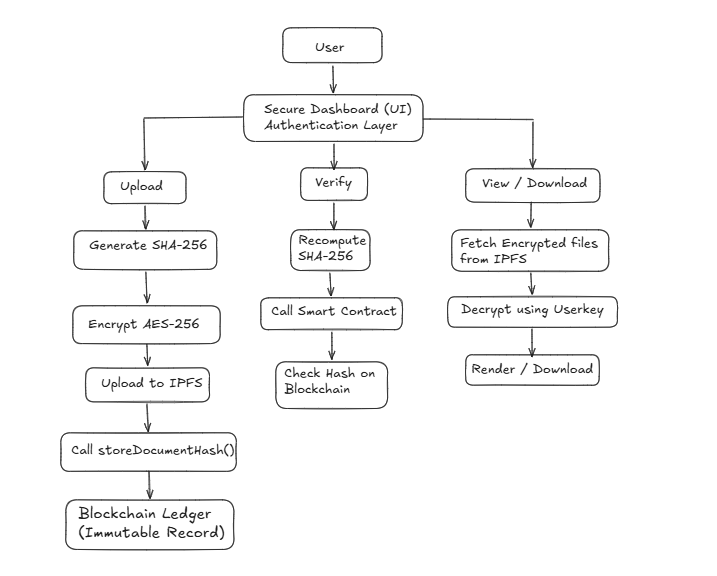
\includegraphics[width=15cm]{photos/flowChart.png}
\caption{Control flow of Blockchain Secure Vault}
\label{fig:flowchart}
\end{figure}
\newpage
\section{Testing Module}

This section describes the testing techniques proposed for validating the Blockchain Secure Document Vault system. The objective of testing is to ensure correctness, security, reliability, and performance of all system components including smart contracts, backend services, encryption mechanisms, and dashboard functionality.

\subsection{Proposed Testing Techniques}

To ensure comprehensive system validation, the following testing strategies will be used.

\subsubsection{Unit Testing}

Unit testing is performed to validate individual components and functions independently.

\textbf{Modules Covered:}
\begin{itemize}
\item SHA-256 hashing function
\item AES-256 encryption and decryption
\item JWT authentication logic
\item OTP verification logic
\item Smart contract functions (\texttt{storeDocumentHash}, \texttt{verifyDocumentHash})
\end{itemize}

\textbf{Purpose:}  
To ensure each function performs accurately in isolation.

\subsubsection{Integration Testing}

Integration testing verifies interaction between connected modules.

\textbf{Interfaces Tested:}
\begin{itemize}
\item Backend API $\leftrightarrow$ Database (MongoDB)
\item Backend API $\leftrightarrow$ IPFS storage
\item Backend API $\leftrightarrow$ Blockchain smart contract
\item Dashboard $\leftrightarrow$ Backend API
\end{itemize}

\textbf{Purpose:}  
To confirm correct data flow and communication between system components.

\subsubsection{Smart Contract Testing}

Smart contract testing ensures on-chain correctness.

\textbf{Scenarios Tested:}
\begin{itemize}
\item Duplicate hash prevention
\item Correct storage of metadata
\item Accurate verification response
\item Transaction reversion on invalid operations
\end{itemize}

\textbf{Purpose:}  
To guarantee immutability and integrity of blockchain records.

\subsubsection{API Testing}

API endpoints are tested using tools such as Postman.

\textbf{Validation Includes:}
\begin{itemize}
\item Correct status codes (200, 401, 403, 409, 500)
\item Input validation
\item Error handling
\item Response format verification
\end{itemize}

\textbf{Purpose:}  
To ensure reliable backend services.

\subsubsection{Security Testing}

Security testing validates access control and protection mechanisms.

\textbf{Checks Include:}
\begin{itemize}
\item Unauthorized access denial
\item Invalid or expired JWT token rejection
\item Role-based access enforcement
\item Proper key-handling behavior (no server-side key storage)
\end{itemize}

\textbf{Purpose:}  
To protect against unauthorized access and data breaches.

\subsubsection{End-to-End (E2E) Testing}

Simulates real user workflows.

\begin{itemize}
\item Register $\rightarrow$ Verify OTP $\rightarrow$ Login
\item Upload $\rightarrow$ Encrypt $\rightarrow$ Store $\rightarrow$ Record on blockchain
\item Verify document authenticity
\item View and download document
\item Share and revoke access
\end{itemize}

\textbf{Purpose:}  
To validate complete system functionality under realistic scenarios.

\subsubsection{Performance and Load Testing}

System performance is evaluated under:

\begin{itemize}
\item Multiple concurrent uploads
\item Multiple verification requests
\item Large file uploads (within allowed limit)
\end{itemize}

\textbf{Purpose:}  
To measure system responsiveness and stability.

\subsubsection{Usability and Compatibility Testing}

Dashboard is tested on:

\begin{itemize}
\item Google Chrome
\item Mozilla Firefox
\item Microsoft Edge
\item Mobile and desktop viewports
\end{itemize}

\textbf{Purpose:}  
To ensure consistent user experience across platforms.

\subsection{System Test Cases}

The following test cases will be executed to validate system functionality.

\begin{itemize}

\item \textbf{TC01 -- User Registration (Valid Case)} \\
Input: Valid full name, username, email, password \\
Expected Result: Account created, OTP sent, user marked as unverified.

\item \textbf{TC02 -- OTP Verification (Valid Case)} \\
Input: Correct OTP within expiry period \\
Expected Result: Email verified successfully and login permitted.

\item \textbf{TC03 -- Login (Invalid Password)} \\
Input: Correct username with incorrect password \\
Expected Result: 401 Unauthorized response, no JWT issued.

\item \textbf{TC04 -- Access Protected API Without Token} \\
Input: Request to secured endpoint without JWT \\
Expected Result: 401 Unauthorized error.

\item \textbf{TC05 -- Upload Valid File} \\
Input: Supported file (e.g., PDF within size limit) \\
Expected Result:
\begin{itemize}
\item SHA-256 generated
\item AES-256 encryption completed
\item File uploaded to IPFS
\item Hash recorded on blockchain
\item Decryption key displayed once
\end{itemize}

\item \textbf{TC06 -- Upload Duplicate File} \\
Input: Same file uploaded again \\
Expected Result: Upload rejected with duplicate error; no second blockchain entry created.

\item \textbf{TC07 -- Upload Unsupported File Type} \\
Input: Unsupported extension \\
Expected Result: Validation failure with appropriate error message.

\item \textbf{TC08 -- Verify Authentic Document} \\
Input: Previously uploaded original file \\
Expected Result: Hash matches blockchain record; document marked as verified.

\item \textbf{TC09 -- Verify Tampered or Unknown Document} \\
Input: Modified file or never-uploaded file \\
Expected Result: Verification fails; document marked invalid or not found.

\item \textbf{TC10 -- Dashboard View (Correct Key)} \\
Input: Valid document with correct decryption key \\
Expected Result: Successful decryption and document preview.

\item \textbf{TC11 -- Dashboard View (Incorrect Key)} \\
Input: Valid document with wrong decryption key \\
Expected Result: Decryption fails; file not rendered.

\item \textbf{TC12 -- Download Document (Authorized)} \\
Input: Valid key for owned/shared document \\
Expected Result: Original decrypted file downloaded successfully.

\item \textbf{TC13 -- Unauthorized Document Access} \\
Input: User attempts to access unshared document \\
Expected Result: 403 Forbidden or 404 Not Found response.

\item \textbf{TC14 -- Share Document} \\
Input: Owner shares document with valid registered user \\
Expected Result: Share record created; recipient can access document.

\item \textbf{TC15 -- Revoke Shared Access} \\
Input: Owner revokes access \\
Expected Result: Recipient can no longer view or download document.

\item \textbf{TC16 -- Smart Contract Immutability Check} \\
Input: Attempt to overwrite existing hash \\
Expected Result: Transaction reverted; original data unchanged.

\item \textbf{TC17 -- IPFS or Service Failure Handling} \\
Input: Simulated IPFS unavailability \\
Expected Result: Graceful error response; no inconsistent records created.

\item \textbf{TC18 -- Expired or Blacklisted Token} \\
Input: Expired or invalid JWT token \\
Expected Result: Request denied; user redirected to login.

\end{itemize}
\newpage
\section{Performance of the Project (Developed So Far)}

At the current stage of development, the system demonstrates stable functional performance across the core modules that have been implemented so far, including user authentication and secure document upload with encryption and storage. These modules are functioning reliably under normal testing conditions and allow users to interact with the system without major delays or interruptions.

The frontend interface is responsive and provides clear feedback during operations. Loading indicators and error messages are displayed during processes such as authentication and file upload. This improves the user experience by keeping users informed about the progress of their actions.

The backend APIs responsible for handling authentication and document upload workflows are functioning correctly. The system successfully processes file uploads, performs SHA-256 hash generation, and encrypts files using the AES-256 encryption standard before storing them in decentralized storage. The integration between the frontend, backend, and storage components is working consistently for the currently implemented features.

The blockchain integration for storing document hash records has also been established. However, blockchain-related operations may take slightly more time compared to traditional database operations because transactions must be confirmed on the network. This delay is expected and acceptable within the scope of a blockchain-based system.

From a security-performance perspective, cryptographic operations such as hash generation and encryption introduce some computational overhead. Despite this, the system performance remains acceptable for the current prototype scale and does not create noticeable delays during testing.

Based on the tests conducted so far, no major performance bottlenecks have been observed in the implemented modules. The system can therefore be considered stable for prototype-level functionality at this stage of development.

\subsection{Conclusion}

The implemented system demonstrates satisfactory performance for the currently developed modules, particularly in authentication, secure document processing, and encrypted storage. Additional features and further performance evaluation will be conducted in later stages of development.
\newpage

\section{Output Screen}
\begin{figure}[H]
\centering
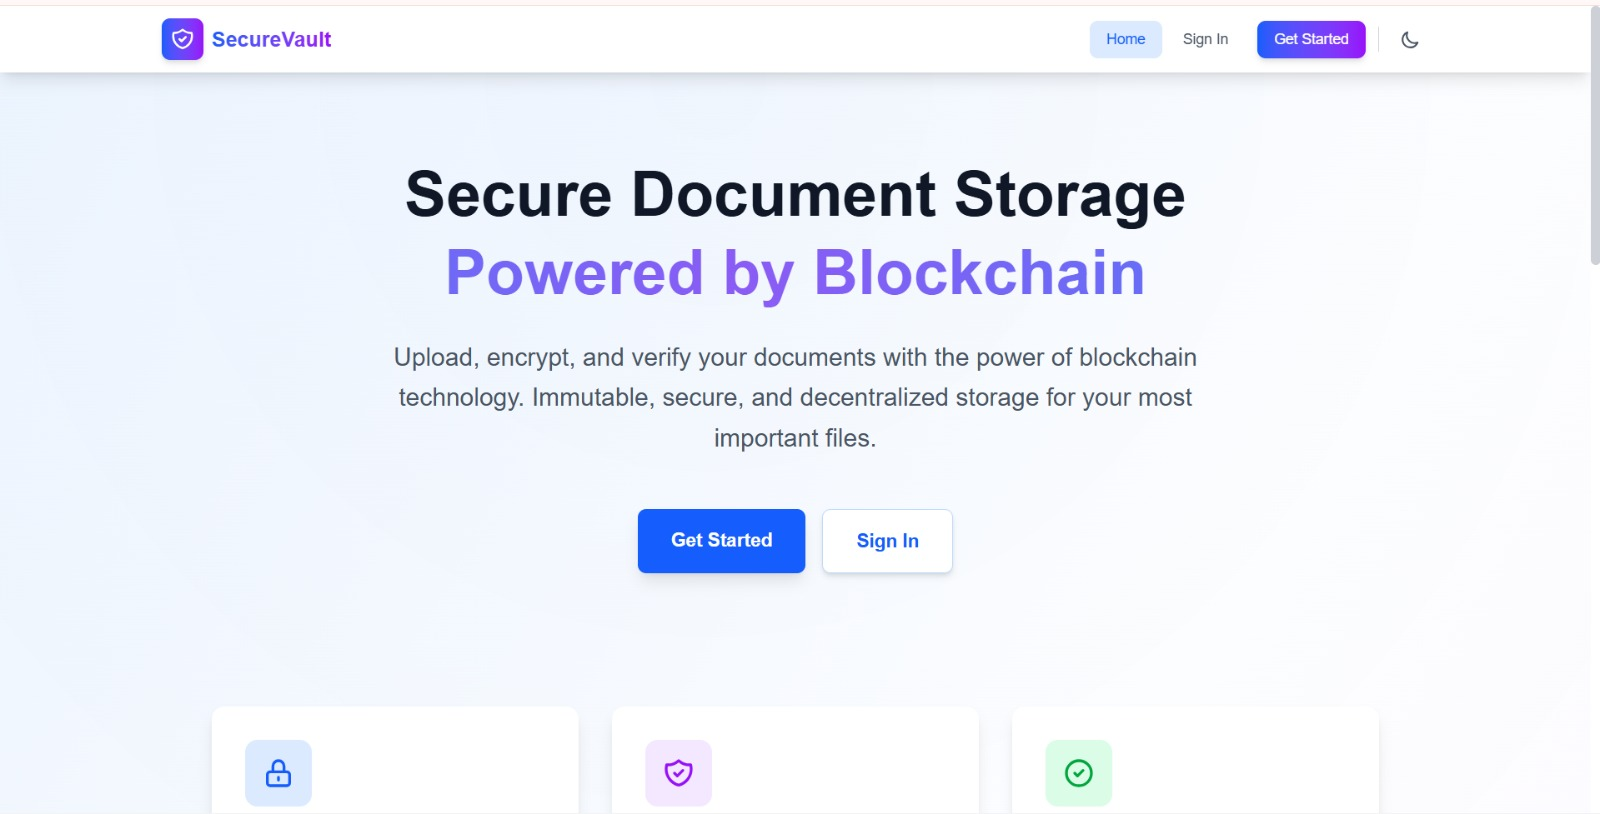
\includegraphics[width=15cm]{photos/one.jpeg}
\caption{Landing page of the system before user authentication}
\label{fig:one}
\end{figure}

\begin{figure}[H]
\centering
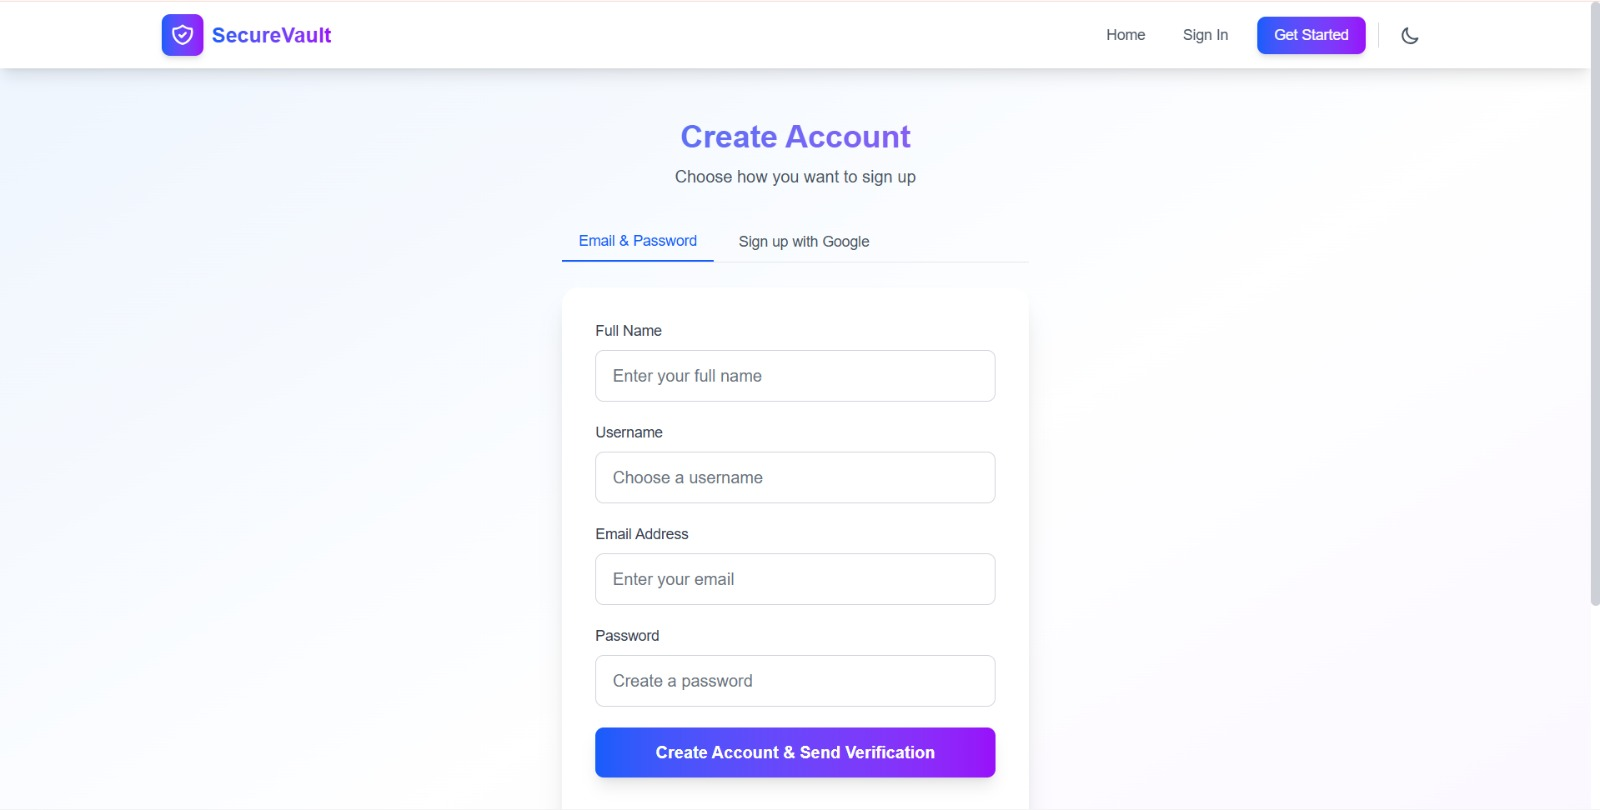
\includegraphics[width=15cm]{photos/two.jpeg}
\caption{User registration interface for creating a new account}
\label{fig:two}
\end{figure}

\begin{figure}[H]
\centering
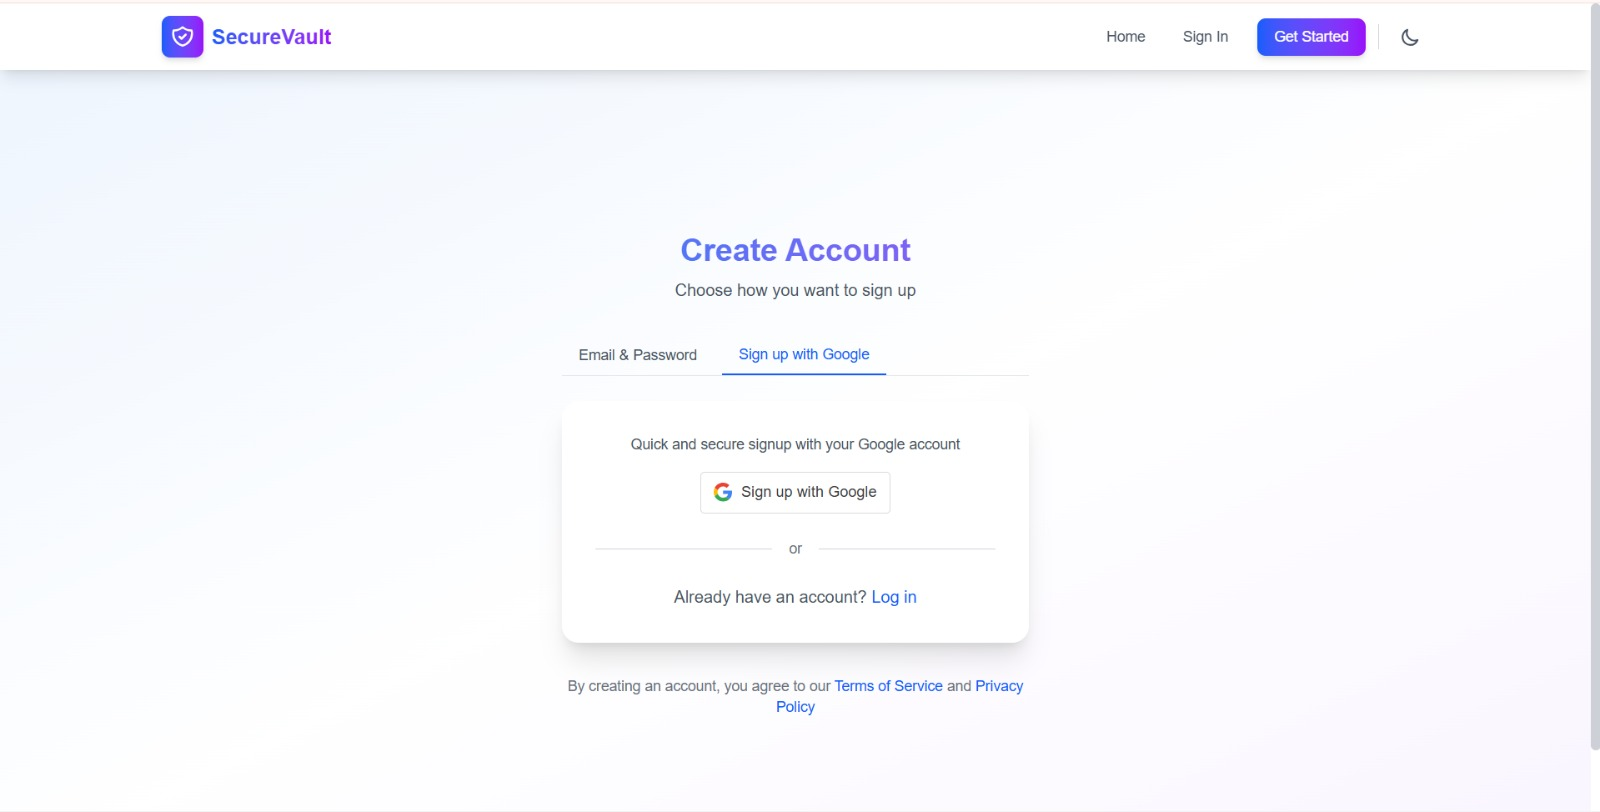
\includegraphics[width=15cm]{photos/three.jpeg}
\caption{Account registration using Google authentication}
\label{fig:three}
\end{figure}

\begin{figure}[H]
\centering
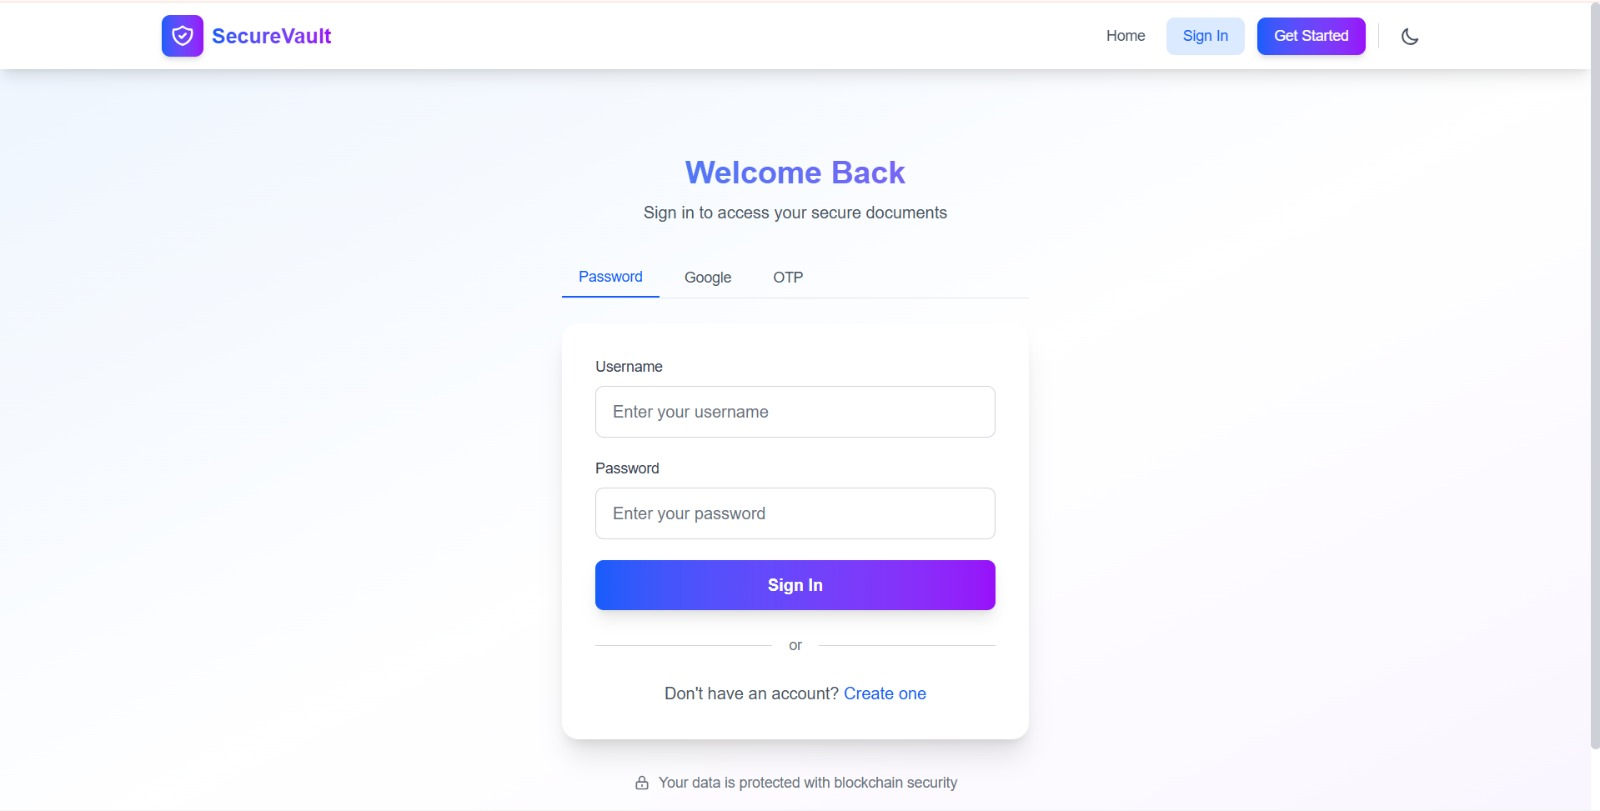
\includegraphics[width=15cm]{photos/four.jpeg}
\caption{User login interface using username and password}
\label{fig:four}
\end{figure}

\begin{figure}[H]
\centering
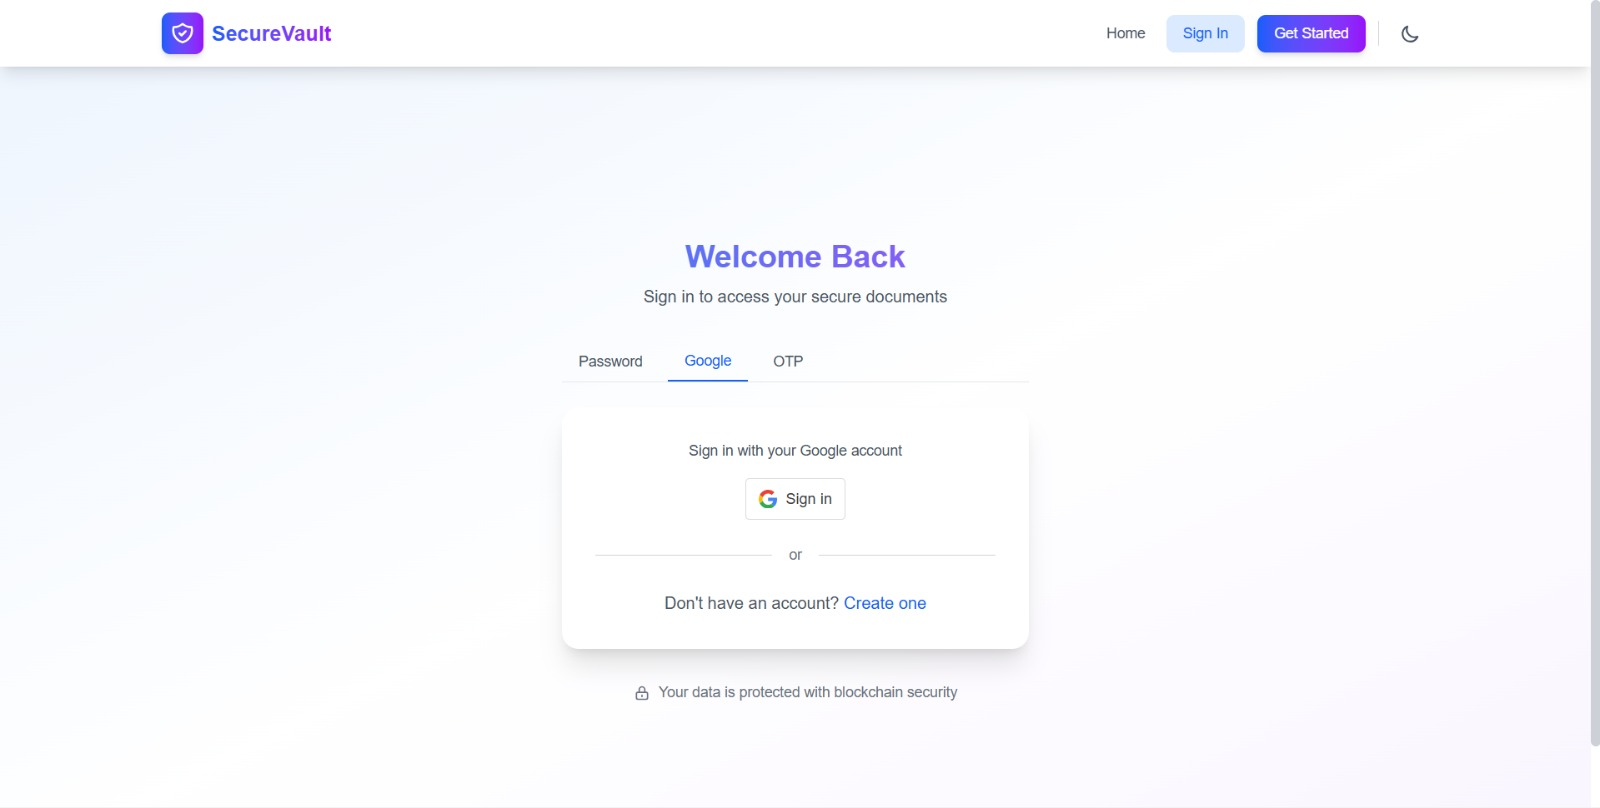
\includegraphics[width=15cm]{photos/five.jpeg}
\caption{User login using Google authentication}
\label{fig:five}
\end{figure}

\begin{figure}[H]
\centering
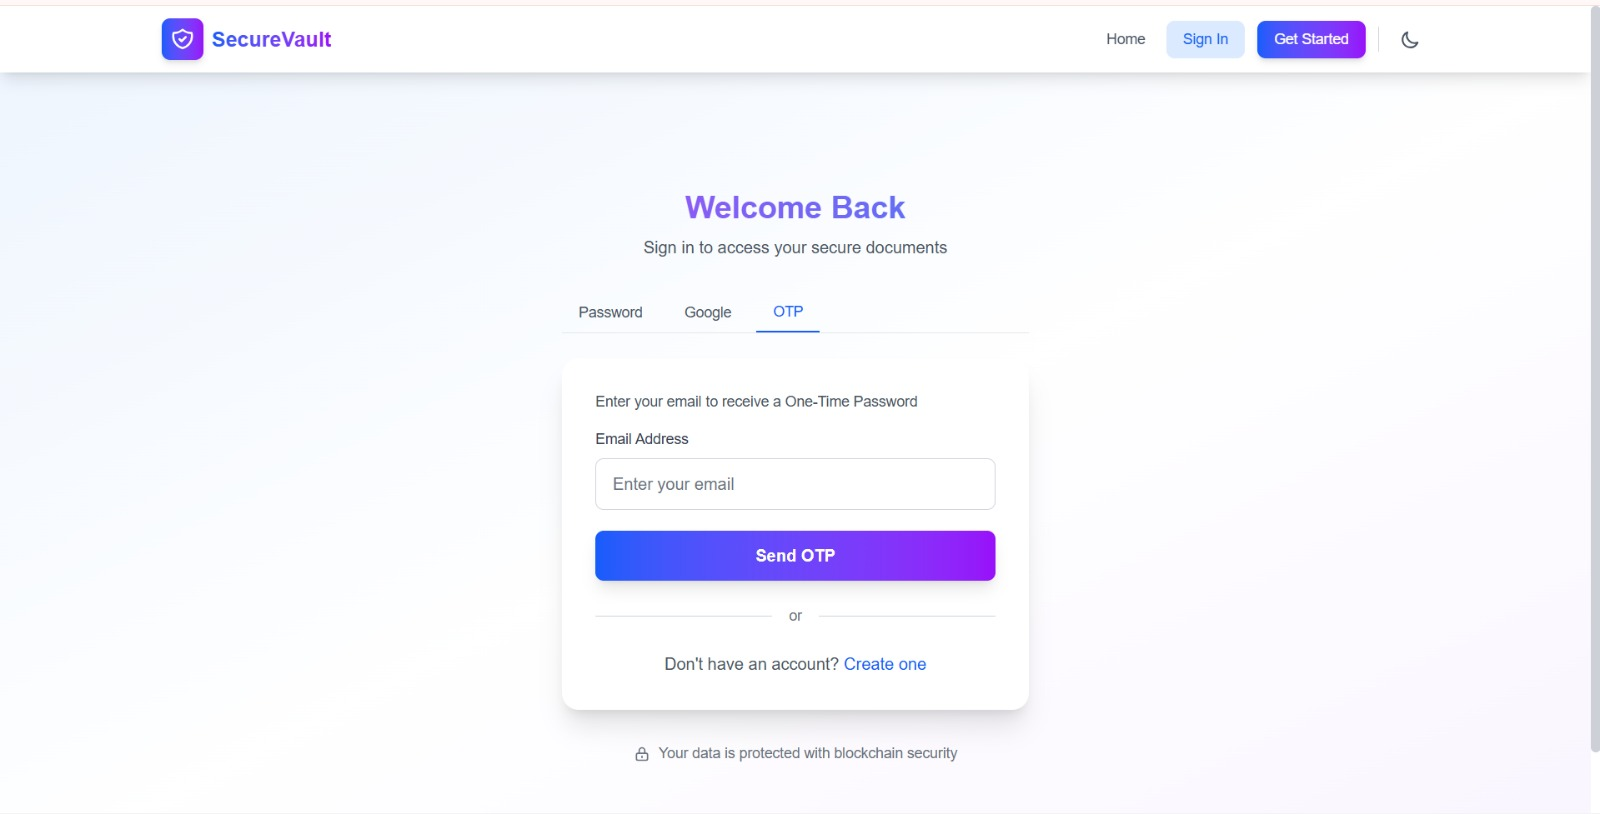
\includegraphics[width=15cm]{photos/six.jpeg}
\caption{User login using One-Time Password (OTP) verification}
\label{fig:six}
\end{figure}



\begin{figure}[H]
\centering
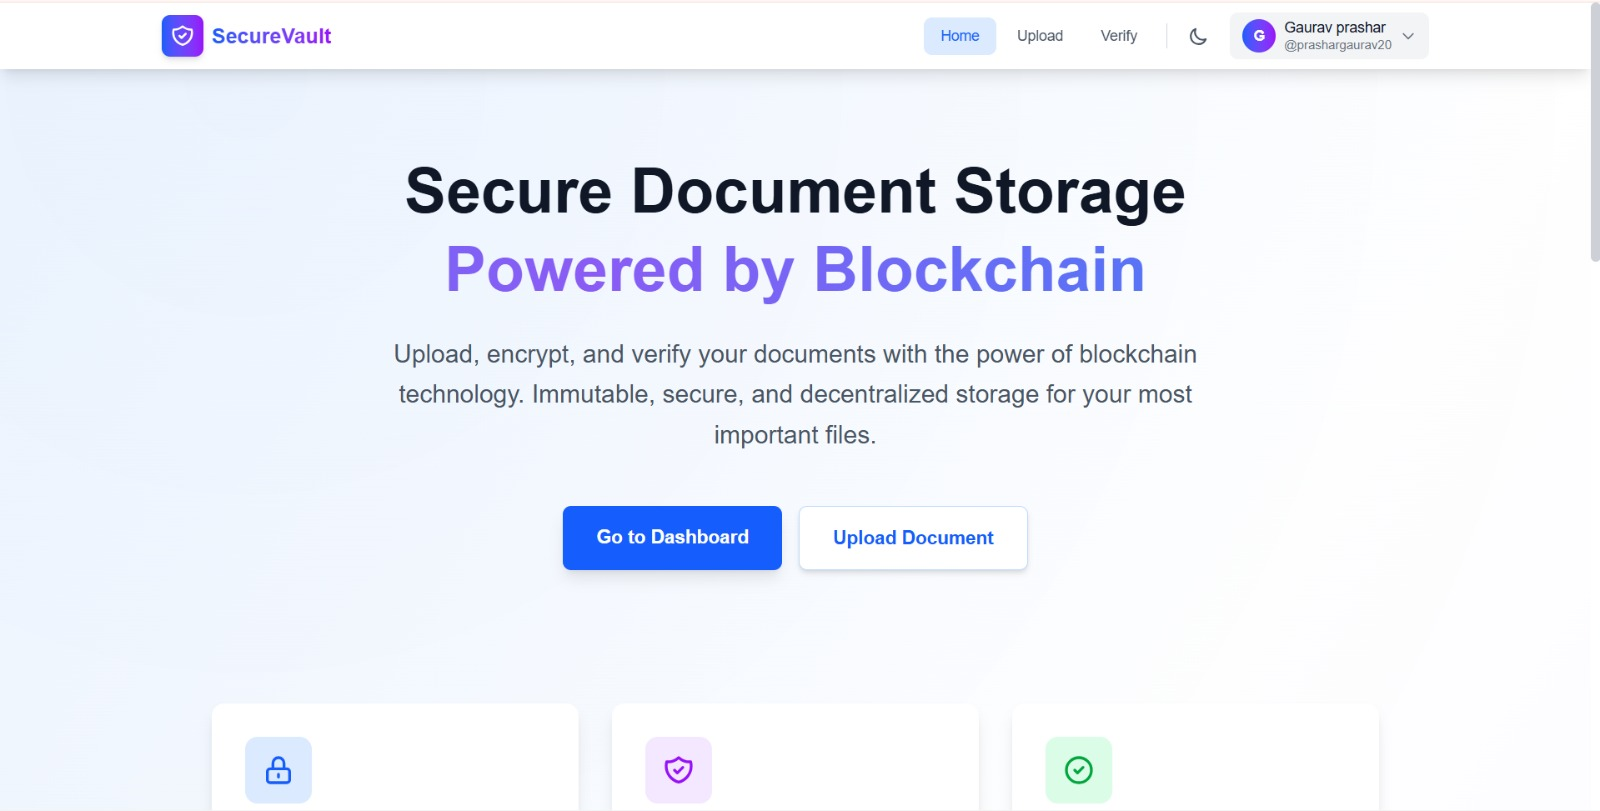
\includegraphics[width=15cm]{photos/nine.jpeg}
\caption{Home interface displayed after user authentication}
\label{fig:nine}
\end{figure}

\begin{figure}[H]
\centering
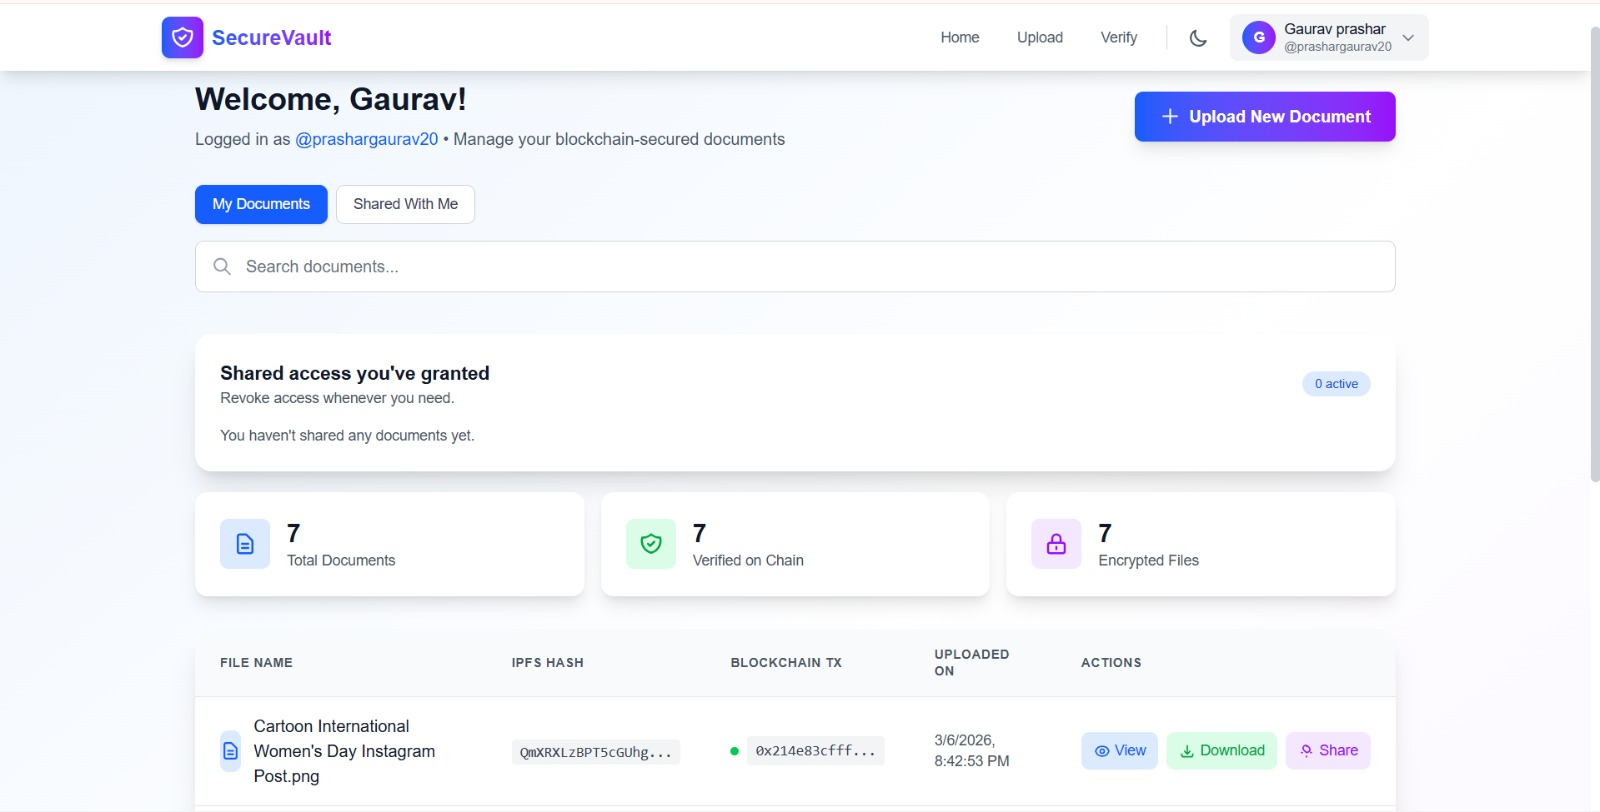
\includegraphics[width=15cm]{photos/eight.jpeg}
\caption{Secure document management dashboard after successful login}
\label{fig:eight}
\end{figure}

\begin{figure}[H]
\centering
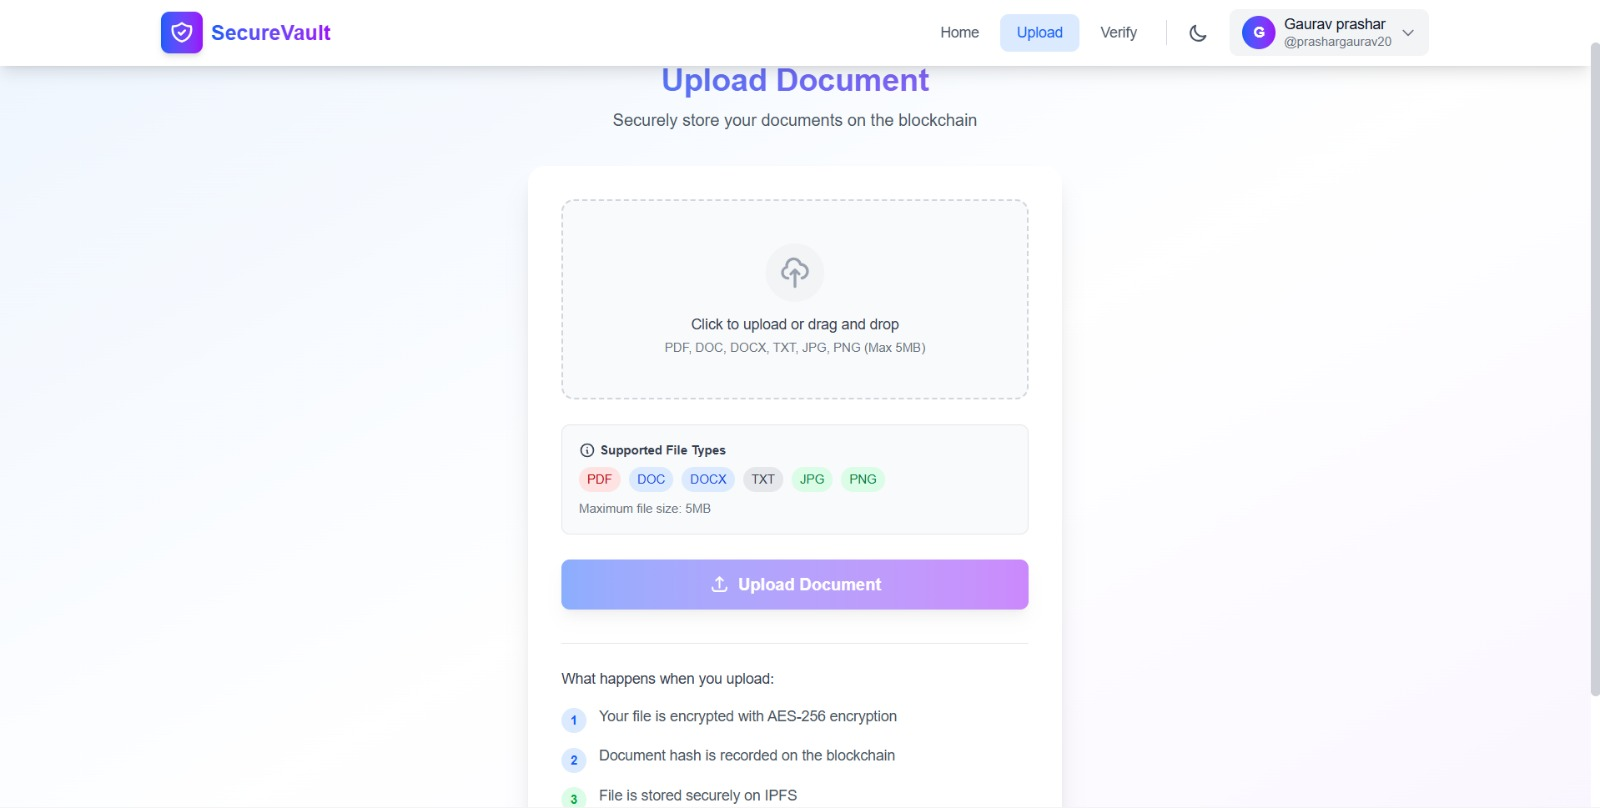
\includegraphics[width=15cm]{photos/ten.jpeg}
\caption{Document upload interface for secure file encryption and storage}
\label{fig:ten}
\end{figure}

\begin{figure}[H]
\centering
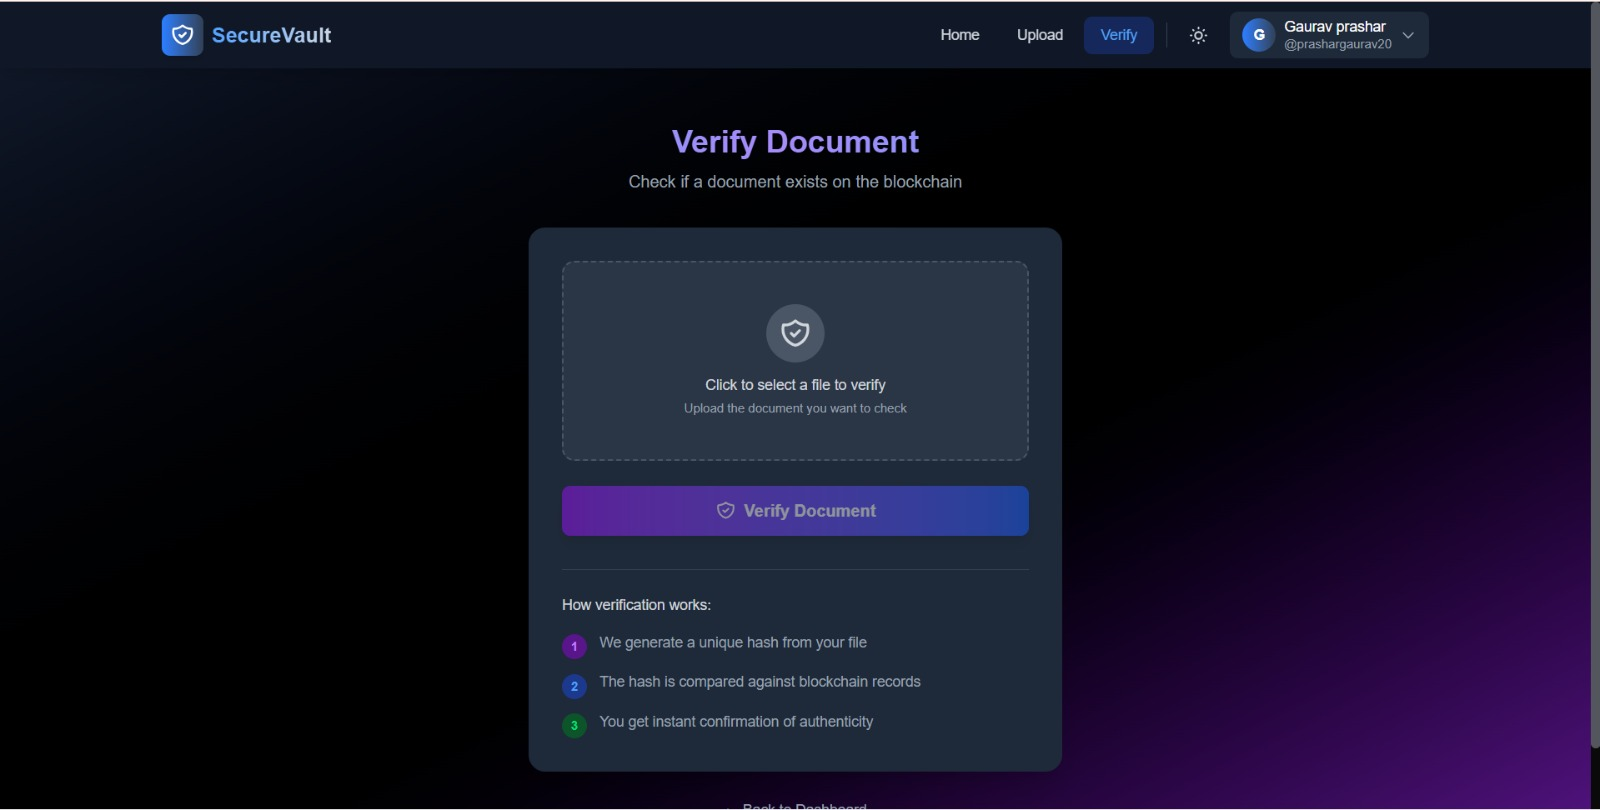
\includegraphics[width=15cm]{photos/eleven.jpeg}
\caption{Document verification interface for validating file authenticity using blockchain records}
\label{fig:eleven}
\end{figure}
\newpage

\bibliographystyle{IEEEtran}
\bibliography{references}

\end{document}
